% ----------------------
  \chapter{Introducción}
% ----------------------
\label{C:introduccion}
Dentro de la Universidad de Costa Rica, cada una de las escuelas de carreras tienen el deber de mantener año tras año un inventario de todos los activos que poseen. Con la cantidad tan grande de estudiantes que se aloja en ella, los materiales requeridos para poder dar una educación de calidad es igual o inclusive mayor, por lo que un inventario puede llegar a tomar bastante tiempo y requerir de múltiples personas que lo hagan. Automatizar el proceso de inventariado en algún nivel conllevaría a una reducción significativa de la carga que esto conlleva.
\par
Una de las herramientas que actualmente se utiliza para poder automatizar muchas tareas en el campo laboral y cotidiano, es la inteligencia artificial, más específicamente las redes neuronales. Al tener la capacidad de resolver problemas, realizar tareas, hacer cálculos entre otras aplicaciones, así como la capacidad de aprender constantemente conforme obtienen un buen o un mal resultado, resultan una herramienta muy útil para automatizar procesos.
\par
En el presente trabajo, se busca realizar una aplicación directa de una red neuronal, que logre recibir imágenes tomadas de las placas de los activos, para extraer el número en ellas y registrarla en conjunto con otros datos que los describan. Además se pretende encapsular la aplicación por medio de una aplicación para dispositivos Android, que permita el fácil uso del escáner de placas.

\section{Alcances}
Para poder tener un desarrollo debido del proyecto, primeramente se investigará sobre las redes neuronales: como aplicarlas, como crearlas y como entrenarlas. Además es importante ver que servicios web brindan una red neuronal pre-hecha, para poder simplificar el desarrollo y además evitar falta de recursos computacionales avanzados para un buen funcionamiento de la aplicación. 
\par
Por otro lado se estudiará cómo desarrollar una aplicación móvil sencilla para Android, por medio del lenguaje de programación python. Así mismo, es necesario estudiar los módulos de visión por computador para poder hacer uso de las cámaras de los móviles, módulos de conexión a servidores y por último como almacenar en bases de datos desde las aplicaciones para poder guardar los datos de los activos.
\par
Finalmente con todos estos conceptos estudiados e interiorizados se podrá entrenar a la red neuronal, mientras que se desarrolla una interfaz gráfica para Android, que tome las capturas, envíe a la red para su lectura y permita almacenar los datos en un servidor remoto.

\section{Justificación}
El trabajo de inventariado puede conllevar mucho esfuerzo y tiempo que, cualquier tipo de facilitación sería de gran ayuda. 
\par
La Escuela de Ingeniería Eléctrica al tener una población significativa de estudiantes y un edificio grande, puede tener un proceso de inventario mucho más extenso que otras escuelas, además de que el proceso se realiza año con año.
\par
Bajo estos parámetros se contextualiza el presente proyecto, buscando realizar una herramienta que permita al área administrativa de la EIE una fácil realización de su inventario año tras año. 

\section{Objetivos}
\subsection{Objetivo general}
\begin{itemize}
    \item Desarrollar una aplicación móvil con algoritmos automáticos que facilite el inventario realizado en la escuela.
\end{itemize}
\subsection{Objetivos específicos}
\begin{itemize}
    \item Investigar sobre el aprendizaje automático/redes neuronales, procesamiento de imágenes y aplicaciones móviles en Android.
    \item Diseñar un algoritmo para la detección de números a partir de imágenes correspondientes a placas de activos.
    \item Crear una aplicación móvil que implemente el algoritmo diseñado para el registro de los activos con sus placas.
    \item Crear una interfaz amigable y sencilla de usar para el usuario final, para la aplicación. 
    \item Validar el funcionamiento correcto de la aplicación móvil junto con el algoritmo implementado.
\end{itemize}

\section{Metodología}
Con el fin de poder desarrollar el presente proyecto se seguirán los siguientes pasos:
\begin{itemize}
    \item Investigar sobre las redes neuronales y como usarlas para OCR.
    \item Buscar una alternativa basada en web, que permita usar una red neuronal dentro de ella y hacerle envío de archivos para su procesamiento.
    \item Entrenar la red neuronal para pueda detectar los números de las placas de los activos de la escuela.
    \item Aprender a enviar los archivos por medio de un script de python, así como extraer los resultados de los mismos.
    \item Investigar sobre los módulos que permiten crear aplicaciones Android con Python.
    \item Diseñar una interfaz gráfica para Android que integre el algoritmo de la red neuronal
    \item Investigar sobre el almacenamiento de datos por medio de bases de datos.
    \item Hacer que la aplicación almacene los datos coleccionados en una base de datos.
    
\end{itemize}

\section{Cronograma}
\begin{figure}[H]
\centering
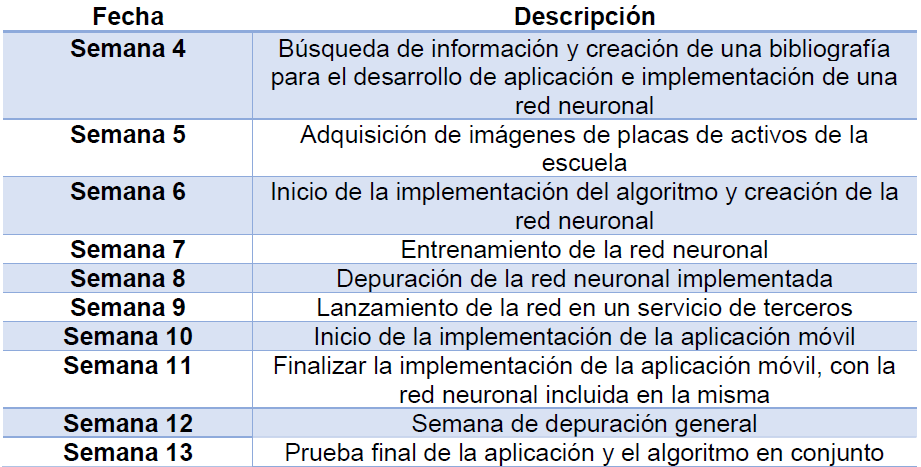
\includegraphics[width=\textwidth]{imagenes/Cronograma.PNG} 
\caption{Cronograma del proyecto eléctrico}
\label{F:crono}
\end{figure}
